\documentclass{standalone}

\usepackage{tikz}
\usepackage{circuitikz}

\tikzset{block/.style = {draw, fill=white, very thick, rectangle, minimum height=1cm, minimum width=2cm},
         lblock/.style={draw,fill=white,very thick, rectangle, minimum height=3cm, minimum width=1cm},
         sum/.style= {draw, fill=white, very thick, circle, node distance=0.5cm}}

         
\begin{document}
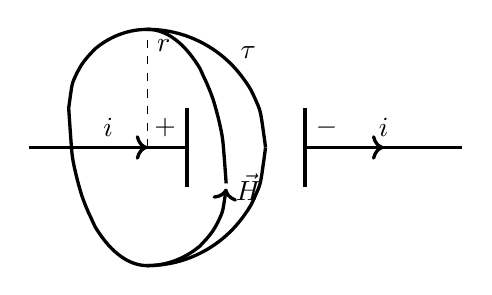
\begin{tikzpicture}[scale=2]
    \draw[-,very thick](-0.75,0)--(0.25,0)node[above left]{$+$};
    \draw[-,ultra thick](0.25,-0.25)--(0.25,0.25);
    \draw[-, very thick](1,0)node[above right]{$-$}--(2,0);
    \draw[-,ultra thick](1,-0.25)--(1,0.25);
    
    \draw[->,very thick](-0.25,0)node[above]{$i$}--(0,0);
    \draw[->,very thick](1.25,0)--(1.5,0)node[above]{$i$};
    \draw[dashed](0,0)--(0,0.75)node[below right]{$r$};

    \node[right]at(0.5,-0.25){$\vec{H}$};
    \node[above left]at(0.75,0.5){$\tau$};

    \draw[->,very thick]plot[smooth, domain=0:0.5](\x,{-0.25-(0.25-(\x)^2)^0.5});
    \draw[-,very thick]plot[smooth, domain=-0.5:0](\x,{+0.25+(0.25-(\x)^2)^0.5});
    \draw[-,very thick]plot[smooth, domain=-0.5:0](\x,{+0.25-2*(0.25-(\x)^2)^0.5});
    \draw[-,very thick]plot[smooth, domain=0:0.5](\x,{-0.25+2*(0.25-(\x)^2)^0.5});
    \draw[-,very thick]plot[smooth, domain=0:0.75](\x,{(0.5625-(\x)^2)^0.5});
    \draw[-,very thick]plot[smooth, domain=0:0.75](\x,{-(0.5625-(\x)^2)^0.5});
\end{tikzpicture}
\end{document}